\documentclass{article}
\usepackage[utf8]{inputenc}
\usepackage[spanish]{babel}
\usepackage{amsmath}
\usepackage{amssymb}
\usepackage{amsfonts}
\usepackage{hyperref}
\usepackage{textcomp}
\usepackage{graphicx}
\usepackage{pgfplots}
\usepackage{geometry}
\hypersetup{
    colorlinks=true,
    linkcolor=black,
    citecolor=green,
    filecolor=magenta,      
    urlcolor=cyan,
}
\geometry{
  top=3cm,            % Margen superior
  bottom=3cm,         % Margen inferior
  left=3cm,           % Margen izquierdo
  right=3cm           % Margen derecho
}

\title{Estadística 1}
\author{Jorge Miguel Alvarado Reyes}
\date{16 Agosto 2023}

\setlength{\parindent}{0pt}
\begin{document}

\begin{titlepage}
    \begin{center}
        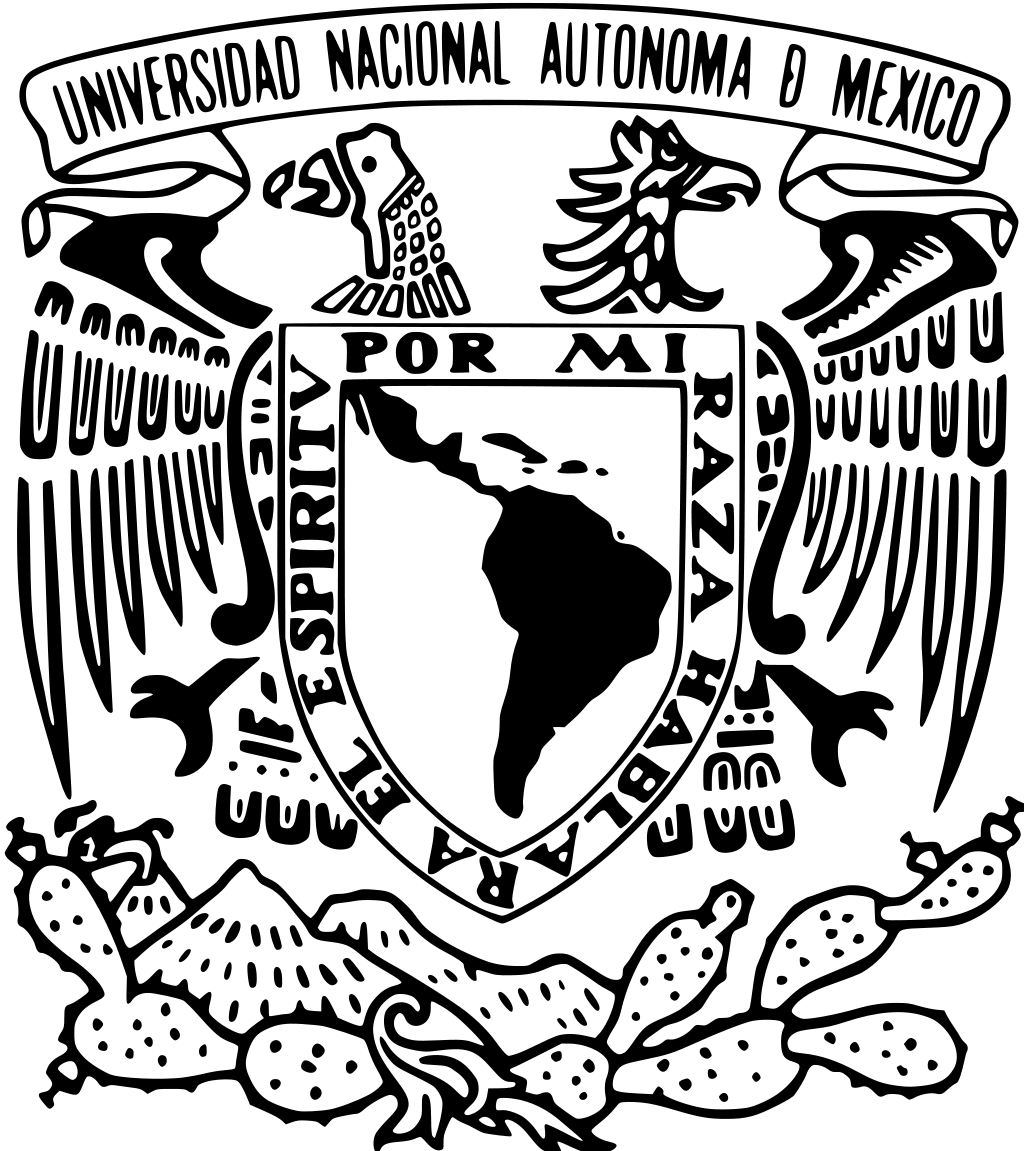
\includegraphics[width=0.2\textwidth]{../../unam.png}
        \vspace*{.5cm}

        \LARGE
        \textbf{Universidad Nacional Autónoma de México}

        \vspace{0.5cm}
        \LARGE
        Facultad de Estudios Superiores Acatlán

        \vspace{2cm}

        \textbf{Apuntes} \\
        Procesos Estocasticos

        \vfill

        \vspace{1cm}

        \textbf{\large Autor:} \\
        Jorge Miguel Alvarado Reyes \\
        \vspace{.5cm}
        \normalsize \today

    \end{center}
\end{titlepage}
\newpage

\tableofcontents

\newpage

\section{Problema 1}

Demuestre que para un $N_n$ definido en un proceso de Bernoulli, la varianza, $\text{Var}(N_n)$, es igual a $npq$
Sea \( X \) el número de éxitos, entonces:
\[ E(N_n) = np \]

Para cualquier \( X_i \):
\[ P(X_i = 1) = p \text{ Exito}\]
\[ P(X_i = 0) = 1 - p = q \text{ Fracaso}\]

Entonces la esperanza de \( X \) es:
\[ E(N_n) = E(X_1) + E(X_2) + \ldots + E(X_n) \]

Para cualquier \( X_i \):
\[ E(X_i) = 0 \cdot q + 1 \cdot p = p \]

Entonces:
\[ E(N_n) = p + p + p \text{ Asi n veces}\]
\[ E(N_n) = np\]

ahora debemos encontrar $E(N_n^2)$

\[E(N_n^2) = \sum_{k=0}^{n} k^2 \cdot P(N_n = k)\]

\[P(N_n = k) = \binom{n}{k} p^k q^{n-k}\]

entonces

\[E(N_n^2) = \sum_{k=0}^{n} \binom{n}{k} p^k q^{n-k}\]

\[E(N_n^2) = npq + (np)^2\]

Entonces la varianza es

\[Var(N_n) = E(N_n^2) - E(N_n)^2\]

\[Var(N_n) = npq + (np)^2 - (np)^2\]

\[Var(N_n) = npq\]

\section{Problema 2}

Demuestre que la funcion generatriz de momentos de la caminata aleatoria es $M(t) = (pe^t + qe^{-t}) * n$. Recuerda que la funcion generatriz de momentos es: $m(t) = E(e^{tx})$


\subsection*{Paso 1: Definición de la Función Generatriz de Momentos}
La función generatriz de momentos $m(t)$ de una variable aleatoria $X$ se define como:
\[ m(t) = E[e^{tX}] \]

\subsection*{Paso 2: Aplicación a la Caminata Aleatoria}
Para un solo paso $X_i$ de la caminata, donde $X_i = +1$ con probabilidad $p$ y $X_i = -1$ con probabilidad $q$, la función generatriz de momentos es:
\[ m_i(t) = E[e^{tX_i}] = pe^{t(+1)} + qe^{t(-1)} = pe^t + qe^{-t} \]

\subsection*{Paso 3: Función Generatriz de Momentos para $n$ Pasos}
Considerando que la caminata aleatoria está compuesta por $n$ pasos independientes y que la función generatriz de momentos para la suma de variables aleatorias independientes es el producto de sus funciones generatriz de momentos individuales, la función generatriz de momentos para la caminata aleatoria completa, $M(t)$, es:
\[ M(t) = (m_i(t))^n = (pe^t + qe^{-t})^n \]


\section{Problema 3}

Demuestre que para $n,k \in \{1,2,3,\dots\}$

\[P\{N_{n+1} = k\} = p * P\{N_n = k-1\} + q * P\{N_n = k\}\]

donde $N_n$ es el número de éxitos en $n$ ensayos de Bernoulli, $p$ es la probabilidad de éxito, y $q = 1 - p$ es la probabilidad de fracaso.

Utilizando la ley de probabilidad total:
\[ P\{N_{n+1} = k\} = P\{N_{n+1} = k | N_n = k-1\} \cdot P\{N_n = k-1\} + P\{N_{n+1} = k | N_n = k\} \cdot P\{N_n = k\} \]

En un ensayo solo puede ocurrir un éxito o un fracaso:
\[ P\{N_{n+1} = k | N_n = k-1\} = p \]
\[ P\{N_{n+1} = k | N_n = k\} = q \]

La fórmula se reduce a:
\[ P\{N_{n+1} = k\} = p \cdot P\{N_n = k-1\} + q \cdot P\{N_n = k\} \]

\section{Problema 4}

Demuestre la formula de probabilidades de transicion de una caminata alaeatoria simple usando ahora los pasos que se dan a la izquierda

\section{Problema 5}

Para una caminata aleatoria simple \(X_n\) sobre los enteros, demuestre que:
\[ P(X_{n+1} = x) = pP(X_n = x - 1) + qP(X_n = x + 1) \]

Sugerencia: Sustituya los parámetros de las probabilidades en la fórmula de probabilidades de transición de una caminata aleatoria y con álgebra verifique la igualdad.

\section{Problema 6}

Una partícula realiza una caminata aleatoria simétrica sobre los enteros empezando en 0. Encuentre la probabilidad de que la partícula no se encuentre nuevamente en el origen en el sexto paso.

\section{Practica 2}

\subsection*{Problema 1}

Considere que existe una partícula que realiza una caminata aleatoria sobre los números enteros, iniciando en 3. La probabilidad de dar un paso a la derecha es de \( \frac{2}{3} \). Encuentre la probabilidad de que la partícula se encuentre:

\begin{enumerate}
    \item[a)] En la posición 8 en 10 pasos.
    \item[b)] Regrese a la posición 3 en 6 pasos.
\end{enumerate}

\subsection*{Problema 2}

Considere una partícula que realiza una caminata aleatoria simple simétrica sobre los enteros. Encuentre la probabilidad de que la partícula se encuentre:

\begin{enumerate}
    \item[a)] En la posición 5 en 9 pasos.
    \item[b)] En la posicion 3 o 7 en 10 pasos
    \item[c)] En la posicion 2 en 7 pasos 
\end{enumerate}


\end{document}